The dynamic project naming script in the code listing for the \texttt{adoe}
code example is shown in Figure \ref{fig:naming-code-adoe}.  This is used to create a project with the naming convention:\\\\
\texttt{<first 6 or less chars of collection>\_<project name>\_<repo name>}\\

In this example, an authenticated API call is made to retrieve the collection name
for the collection id provided in the event context.

\begin{figure}[h]
    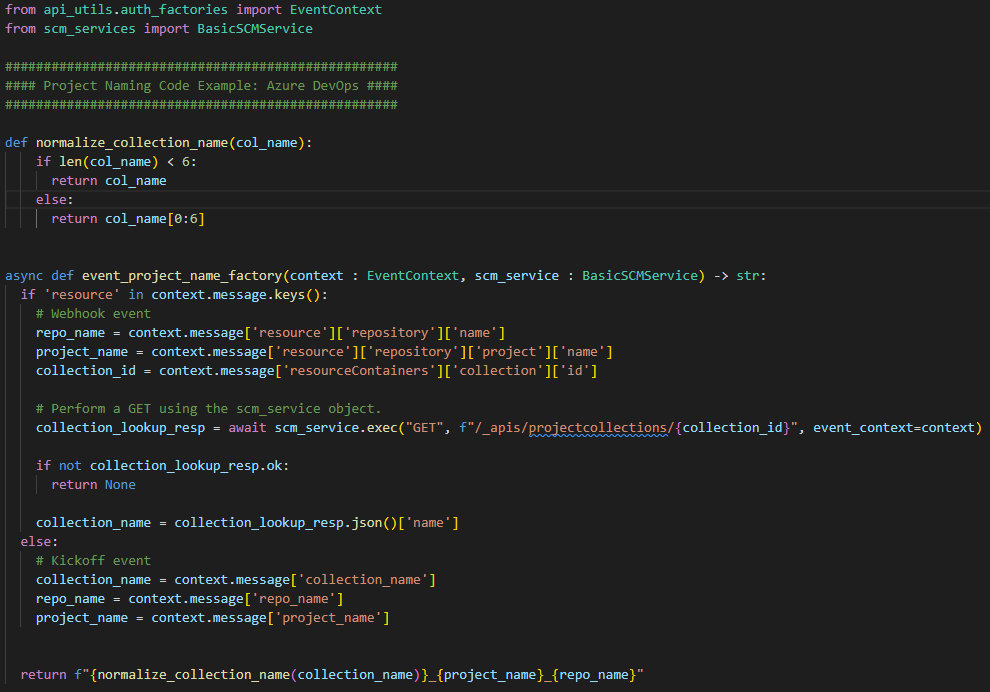
\includegraphics[width=\textwidth]{graphics/naming-code-adoe.png}
    \caption{Azure DevOps Custom Project Naming Code Example}
    \label{fig:naming-code-adoe}
\end{figure}
